\section{Post-Training}
\label{section_post_training}
The post-training phase of Ling 2.0 is engineered to forge a powerful and versatile foundation model—capable of strong reasoning in complex scenarios while maintaining high efficiency for everyday queries. As illustrated in Figure~\ref{fig:post_training}, the process employs a structured three-stage methodology supported by a scalable, high-throughput reward computation infrastructure.

\begin{figure}[htp]
\centering	
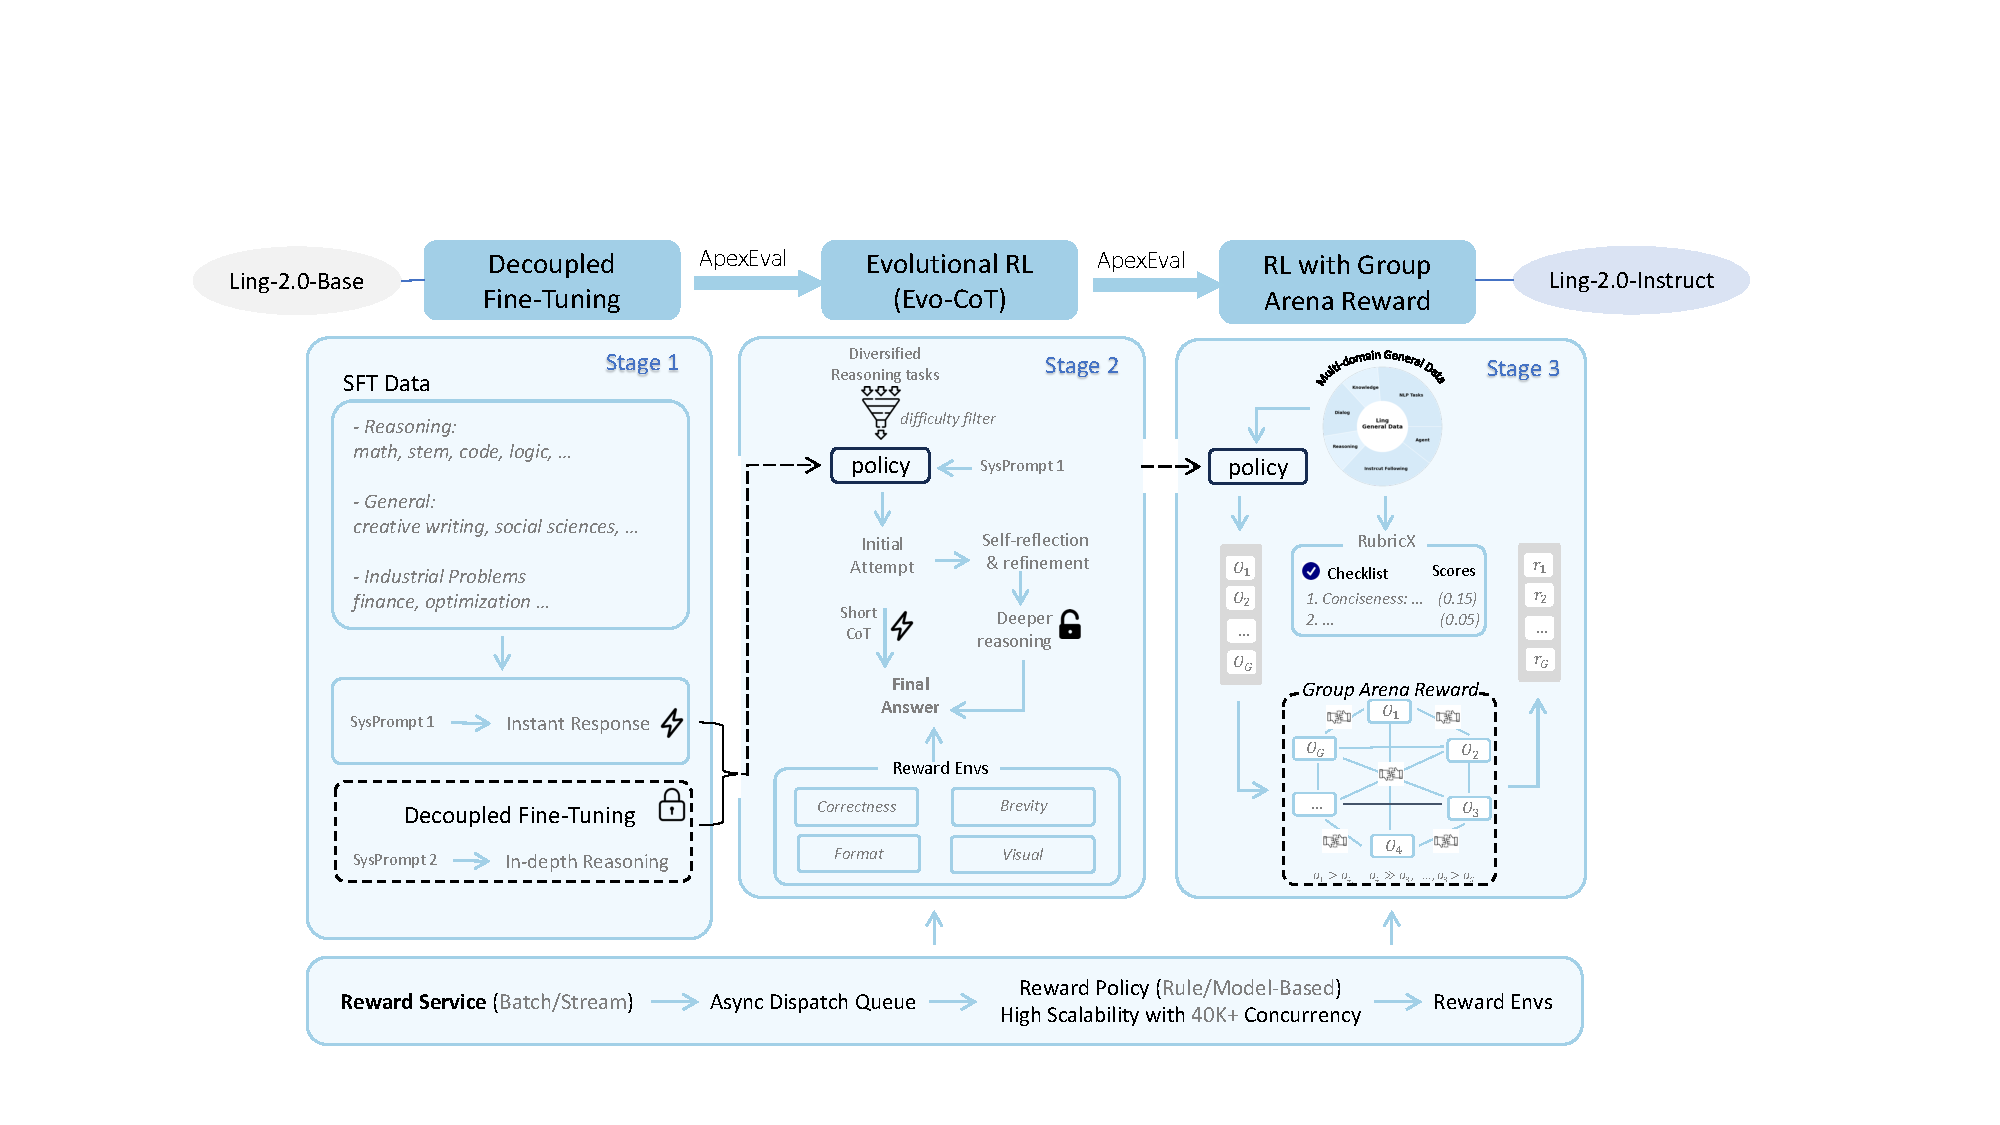
\includegraphics[width=1\textwidth]{figs/posttrain-pipline.pdf}
\caption{Post-training pipeline of Ling 2.0 series models.}
\label{fig:post_training}
\end{figure}


\subsection{Supervised Fine-Tuning with Decoupled Training}
\label{sft}
To create a strong starting point for reinforcement learning (RL), we introduce \emph{Decoupled Fine-Tuning} (DFT)—a supervised approach that constructs training data via differentiated system prompts. As illustrated in Stage~1 of Figure~\ref{fig:post_training}, DFT defines two modes: \textit{Instant Response} (System Prompt~1) and \textit{In-Depth Reasoning} (System Prompt~2), with details provided in Table~\ref{tab:dft_response_modes}. This prompt-guided decoupling enables the model to establish a dedicated deep‑reasoning mode, providing a robust foundation for subsequent RL to further enhance reasoning performance.


\begin{table}[htbp]
  \centering
  \small
  \vspace{0.5cm}
  \caption{Response modes guided by system prompts in Decoupled Fine-Tuning (DFT).}
  \label{tab:dft_response_modes}
  \scalebox{1.1}{%
    \begin{tabular}{@{}lcc@{}}
      \toprule
      & \textbf{Instant Response} & \textbf{In-Depth Reasoning} \\
      \midrule
      \textbf{System Prompt} & detailed think off & detailed think on \\
      \midrule
      & \{response\} & \begin{tabular}{@{}l@{}} 
      \textless think\textgreater \\ 
      \{long-cot\} \\ 
      \textless/think\textgreater \\ 
      \textless answer\textgreater \\ 
      \{response\} \\ 
      \textless/answer\textgreater 
    \end{tabular} \\
      \bottomrule
    \end{tabular}%
  }
\end{table}

\textbf{Balanced, High-Quality SFT Data.}
A balanced capability profile is achieved through a carefully structured SFT dataset integrating multiple task domains under the dual-mode prompt framework. The dataset composition adheres to three principles:
\begin{itemize}
\item \textbf{Reasoning:} mathematical problem solving, stem and logic reasoning, code generation, operations research, and scientific inquiry, ensuring precise logic and analytical depth.
\item \textbf{General:} creative writing, empathetic dialogue, and socio-philosophical discussion, enhancing linguistic richness and social intelligence.
\item \textbf{Industrial:} domain-specific tasks in finance, medical and health, production planning, supply chain orchestration, and transportation optimization, embedding end-to-end workflows under real-world constraints.
\end{itemize}
This integrated design prevents skill imbalance and supports fluent transitions between abstract reasoning and practical problem solving.

\textbf{RL-Potential-Oriented Evaluation.}
Since DFT suppresses explicit chain‑of‑thought, standard accuracy metrics may undervalue its RL potential. We therefore employ \emph{ApexEval} to gauge latent reasoning ability by testing whether problems are solvable under optimal prompting, emphasizing knowledge and reasoning over format‑bound performance. It identifies checkpoints along the stability–improvability frontier to start RL from models that retain responsiveness while maximizing reasoning gains (see Section~\ref{ApexEval}).

\subsection{Evolutionary Reasoning Reinforcement Learning}
\label{ERL}

Building on the DFT-initialized policy, we propose \emph{Evolutionary Chain-of-Thought} (Evo-CoT), a training paradigm designed to instill adaptive reasoning in reflex-grade non-thinking models, enabling them to scale their reasoning depth according to problem complexity.

Formally, Evo-CoT starts from DFT-initialized policy $\pi$ in instant-respsonse mode with system prompt $s_{\text{instant}}$ and evolves its reasoning depth. Given a user query $x$, the policy generates a response $y \sim \pi(\cdot \mid x^{\text{inst}})$ accordingly, where $x^{\text{inst}}$ denotes the concatenation of $(s_{\text{instant}},x)$.
At step $t$, we optimize the policy $\pi$  with parameters $\theta$ via: 
$$\pi_{t+1} = \arg\max_{\pi} \; \mathbb{E}_{x \sim \mathcal{D}} \big[ \mathcal{J}(R(x,y), \theta) - \beta \cdot \mathrm{KL}\big(\pi_\theta(\cdot \mid x^{\text{inst}}) \,\big\|\, \pi_{\text{ref}}(\cdot \mid x^{\text{inst}}\big) \big],$$ 
where $R(\cdot)$ is a composite reward function, $\mathcal{J(\cdot)}$ denotes the RL policy update algorithm detailed in Section \ref{section:lpo}, and $\beta$ controls deviation from the base policy.
The reward consists of:
\begin{itemize}
    \item \textbf{Accuracy} $R_{\text{correctness}}$: +1 if the final answer matches ground truth else 0.
    \item \textbf{Dynamic Length control} $R_{\text{length}}$:  Penalizes exceeding a difficulty-specific length limit with a stage-wise coefficient $\alpha$ that decreases for harder tasks, allowing more elaborate reasoning when needed. 
    \item \textbf{Formatting} $R_{\text{format}}$: if explicit reasoning markers ``\texttt{<think>}'' appear, reward $-0.5$.
    \item \textbf{Task-specific rewards} $R_{\text{task-specific},k}$: optional signals tailored for specific domains (e.g. visual reward for front-end engineering).
\end{itemize}
Taken together, Evo-CoT sustains strong reasoning under complex scenarios while upholding high efficiency for general tasks.

\subsubsection{Tasks-Specific Rewards}
To cater to different domains, we construct a multi‑task reward framework that supports adaptive reasoning across a wide spectrum of tasks.

\textbf{Mathematical, STEM, and Logical Reasoning.}  
Our reward policy is guided by a core principle: \emph{think more about hard problems, respond quickly to easy ones}.  
To implement this principle, we employ the dynamic length control term $R_{\text{length}}$ inspired by \cite{team2025kimi} that encourages brevity for straightforward tasks, while allowing elaborate reasoning for complex ones.  

Formally, we define the \emph{length preference function}:
$$\hat{R}_{\text{length}} =\begin{cases}p(l), & \text{if } r_{\text{acc}} = 1, \\[4pt]\min\!\big(p(l),\, 0\big), & \text{if } r_{\text{acc}} = 0,\end{cases}$$
where
$$p(l) = \left(0.5 - \frac{l - \ell_{\min}}{\ell_{\max} - \ell_{\min} + 10^{-9}}\right).$$
Here, $l_k$ denotes the length (e.g., token count) of the $k$-th sampled response to input $x$, 
$\ell_{\min} = \min_k l_k$ and $\ell_{\max} = \max_k l_k$ represent the shortest and longest responses among the samples, respectively, and $r_{\text{acc}} \in \{0,1\}$ indicates correctness.  

To modulate the influence of the length preference relative to correctness, we introduce a \emph{coefficient} $\alpha > 0$.  
A larger $\alpha$ is used for easier tasks, strongly promoting concise outputs; conversely, a smaller $\alpha$ is applied to harder tasks, thereby encouraging more extensive reasoning.  
In practice, the final scoring function is:
$$R_{\text{length}} = \alpha \cdot \hat{R}_{\text{length}}.$$

This formulation ensures that:
\begin{itemize}
    \item For correct answers, the reward reflects how well the response length aligns with the preferred range.
    \item For incorrect answers, excessively long responses are penalized more, and any positive length-based reward is suppressed.
\end{itemize}
Overall, this design achieves a balance between output accuracy, clarity, and efficiency, while still promoting richer reasoning on challenging problems.

\textbf{Code Reasoning.}
Code reasoning emphasizes functional correctness. We employ a unified reward framework based on test-case execution for code completion, editing, software engineering, and SQL tasks, ensuring reliable functional validation.

\textbf{Front-end Generation.}
For complex front-end engineering tasks, we propose the \emph{Visually Augmented Reward (VAR)} system—at the core of a \emph{Syntax–Function–Aesthetic} triple-filter positive-feedback loop. As shown in Figure~\ref{fig:VAR}, VAR renders generated code into a live interface via a headless browser, then uses a multimodal model to evaluate the screenshot based on aesthetic and usability criteria, yielding a perceptually-aligned reward signal.

\begin{figure}[htp]
\begin{center}	
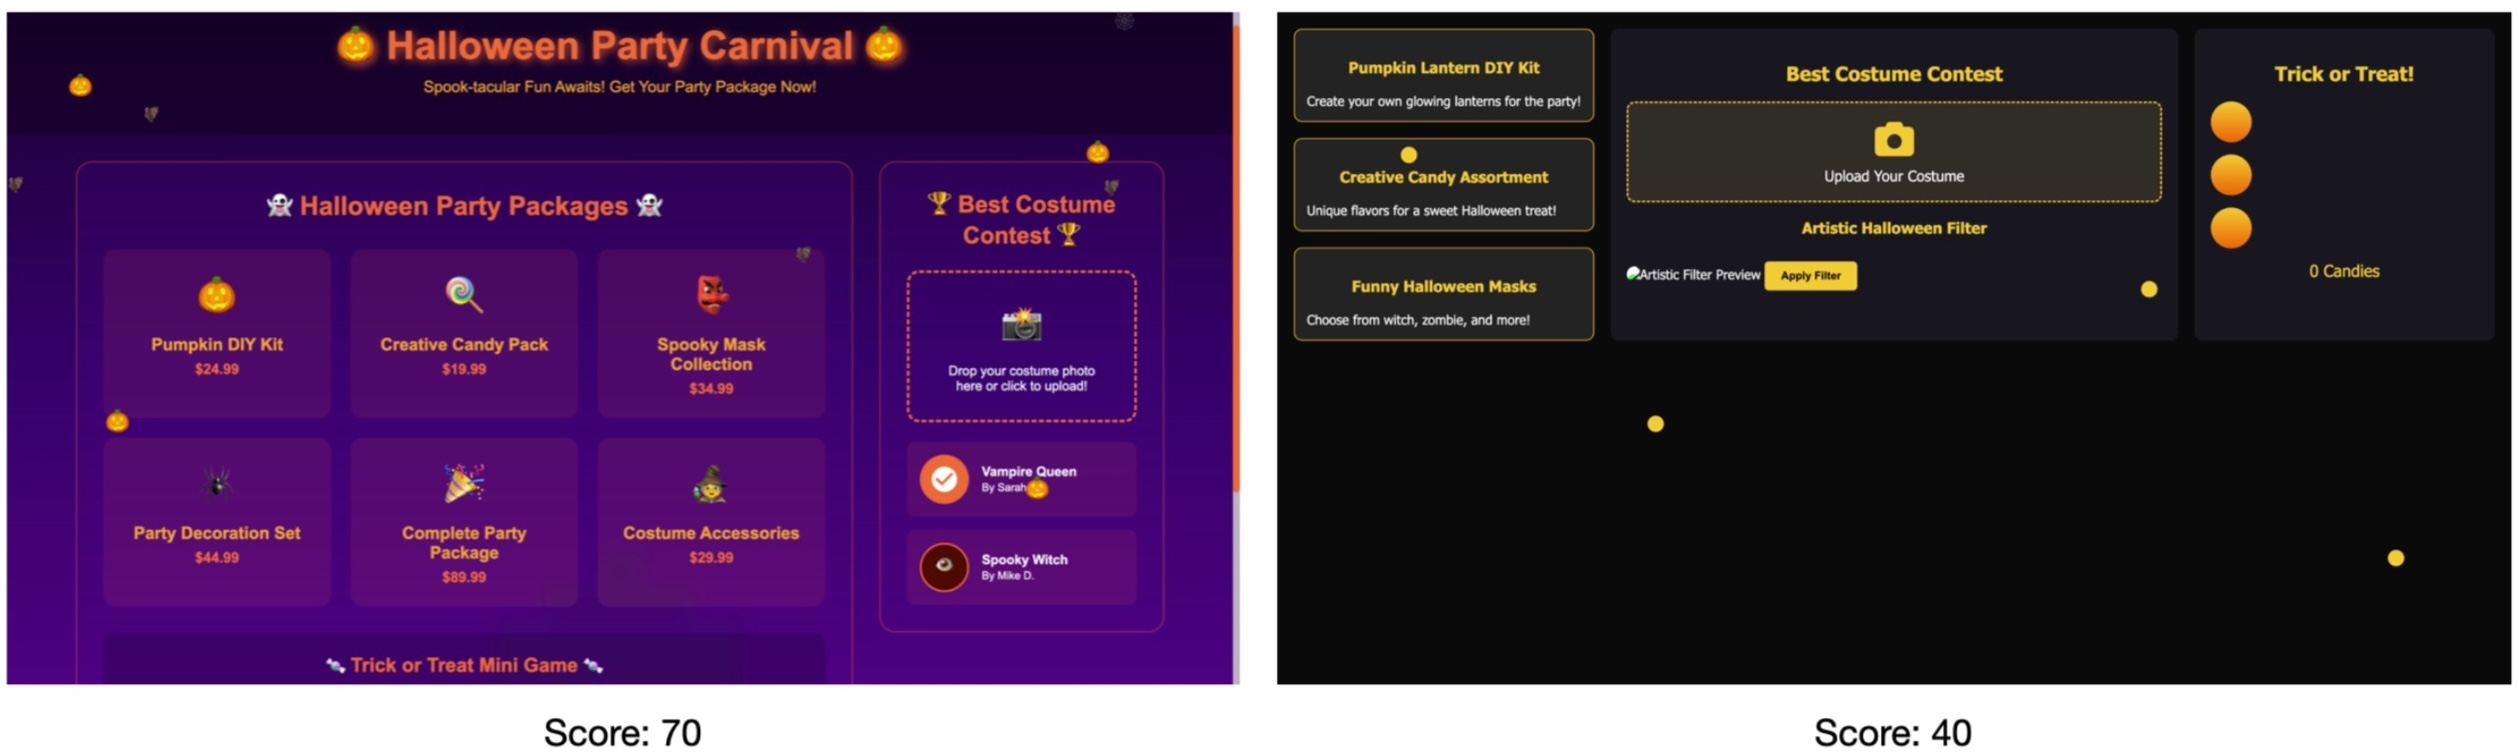
\includegraphics[width=0.9\textwidth]{figs/VAR.jpg}
\end{center}
\caption{A practical example of Visually-Augmented reward. Prompt: "Create an interactive Halloween page with animated background, costume contest upload, candy collection game,
and festive visual effects. Generate clean executable code with smooth interactions."}
\label{fig:VAR}
\end{figure}

\subsubsection{Linguistic-unit Policy Optimization (LPO)}
\label{section:lpo}
We propose \emph{Linguistic-unit Policy Optimization} (LPO), a novel policy gradient algorithm drived by the Evolutionary Chain-of-Thought (Evo-CoT) paradigm. LPO's core mechanism is to perform importance sampling and clipping at the sentence level, defining a linguistic sentence as the fundamental action unit for policy updates. Specifically, Let $\{y_i\}_{i=1}^G$ denote a group of $G$ candidate responses sampled from the old policy 
$\pi_{\theta_{\text{old}}}(\cdot\mid x^{\text{inst}})$. 
For response $y_i$, let $N_{\text{sent}}(y_i)$ denotes the total number of sentences in $y_i$, $s_{i,k}$ the $k$-th sentence in $y_i$ segmented by common pause punctuation marks after detokenization, and $|\cdot|$ denote the token length. The objective function of LPO is formulated as follows:
\begin{equation*}
\scalebox{0.9}{$\displaystyle
\begin{aligned}
\mathcal{J}_{\text{LPO}}(R, \theta)
&= \mathbb{E}_{\{y_i\}_{i=1}^G\!\sim\!
\pi_{\theta_{\text{old}}}(\cdot\mid x^{\text{inst}})}
\left[ 
\frac{1}{\sum_{i=1}^{G}|y_i|} 
\sum_{i=1}^G \sum_{k=1}^{N_{\text{sent}}(y_i)}
|s_{i,k}| \cdot
\min\big(
r_{i,k}(\theta) \, \hat{A}_i,\;
\text{clip}(r_{i,k}(\theta), 1-\varepsilon, 1+\varepsilon) \, \hat{A}_i
\big)
\right],
\end{aligned}
$}
\label{eq:lpo}
\end{equation*}
\noindent
where
\begin{equation*}
\scalebox{0.9}{$\displaystyle
\begin{aligned}
r_{i,k}(\theta) 
&= \exp\left( 
\frac{1}{|s_{i,k}|} 
\sum_{t \in \text{tokens}(s_{i,k})} 
\log \frac{\pi_\theta(y_{i,t} \mid x^{\text{inst}}, y_{i,<t})}{\pi_{\theta_{\text{old}}}(y_{i,t} \mid x^{\text{inst}}, y_{i,<t})} 
\right),\quad
\hat{A_i} = \frac{R(x,y_i) - \text{mean}\left({R(x,y_i)}_{i=1}^G\right)}{\text{std}\left({R(x,y_i)}_{i=1}^G\right)}
\end{aligned}
$}
\label{eq:r-sent}
\end{equation*}
\noindent

LPO performs sentence-level policy updates with the following design choices:
\begin{itemize}
    \item \textbf{Sentence granularity Importance Sampling}: Each sentence $s_{i,k}$ in $y_i$ is treated as an independent action unit, with its importance ratio $r_{i,k}(\theta)$ applied uniformly to all tokens in that sentence.
    \item \textbf{Token-level Normalization}:  Group-based advantage estimation $\hat{A_i}$ are averaged over the total token length $|y_i|$, ensuring scale invariance across examples.
    \item \textbf{Clipping strategy}: Ratios are clipped within $[1-\varepsilon,\, 1+\varepsilon]$ before multiplication, preventing unstable updates while preserving finer granularity than whole-sequence clipping. In our training setting, $\varepsilon=0.03$ .
\end{itemize}
\noindent
This structure aligns the optimization step with the natural semantic boundaries of reasoning, resolving the mismatch in granularity found in conventional token-level and sequence-level methods. It attains stability without sacrificing data efficiency, making LPO a natural fit within the Evo-CoT training paradigm.

Empirically, as shown in Figure~\ref{fig:lpo}, LPO delivers smoother reward curves and markedly greater stability than GRPO~\citep{shao2024deepseekmath}, GSPO~\citep{zheng2025group}, and the GSPO (Token Mean) variant. It avoids plateaus and collapse, converges faster, and generalizes better. On the challenging AIME~2025 test set, LPO-trained models achieve substantially higher accuracy, demonstrating that stabilizing updates at the sentence level not only improves optimization but also guides the policy toward more robust reasoning strategies.

\begin{figure}[h]
\begin{center}	
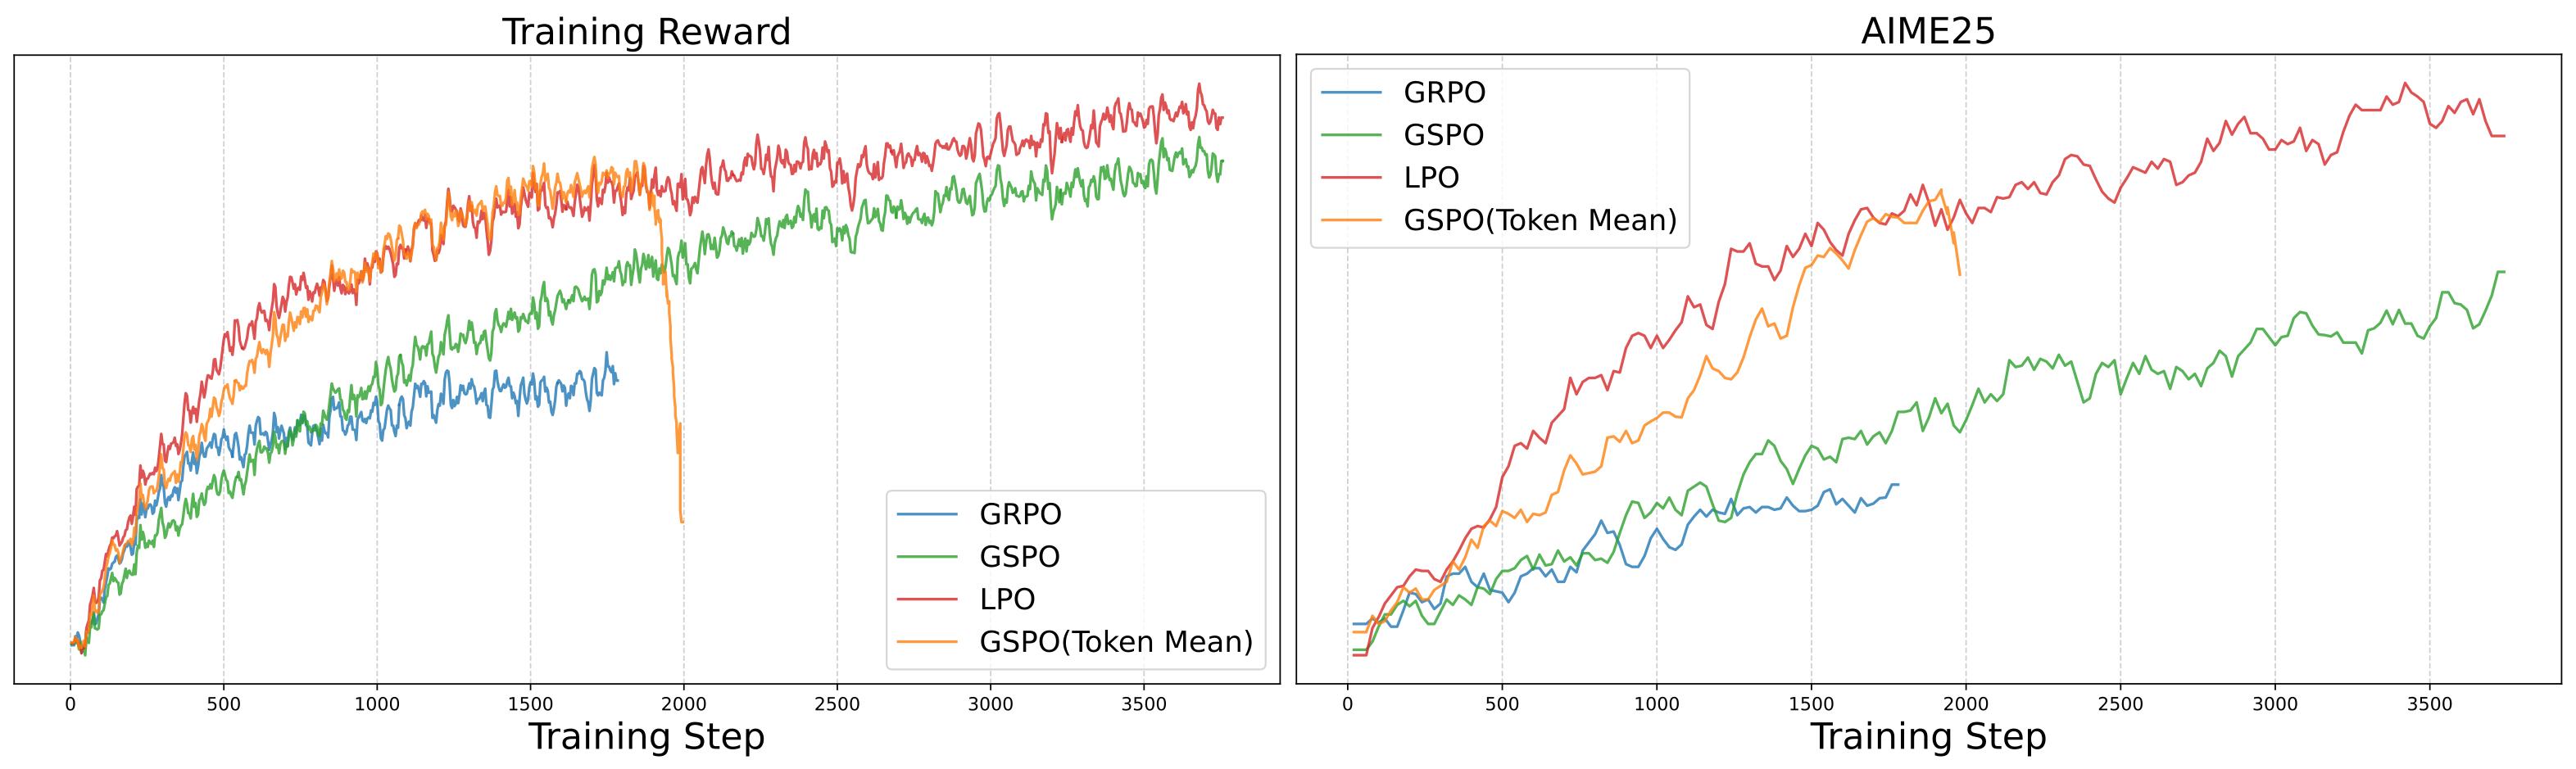
\includegraphics[width=0.95\textwidth]{figs/LPO.png}
\caption{Reward curves of LPO in RL training for the latest Ling~2.0 model. 
Left: reward progression on training data, showing smoother growth and greater stability compared to GRPO~\citep{shao2024deepseekmath}, GSPO~\citep{zheng2025group}, and the GSPO (Token Mean) baseline, with no severe plateaus or collapses. 
Right: reward curves on the AIME~2025 test set, illustrating faster convergence and improved generalization due to sentence-level policy updates.}
\label{fig:lpo}
\end{center}
\end{figure}


\subsection{Group Arena Reward for Human Preference Alignment}
\label{GRL}

In the RLHF post-training stage for open-ended, subjective tasks, two central objectives emerge: 
(1) mitigating reward noise inherent in ambiguous evaluation criteria, and 
(2) aligning model outputs more precisely with nuanced human preferences. 
To this end, we design the \textbf{Group Arena Reward (GAR)} mechanism—an intra-group comparative evaluation strategy—and \textbf{RubriX} (``Rubrics for eXtended domains''), a fine-grained, multi-dimensional reward guideline framework. 
Together, they improve stability in subjective task optimization and enable generation that is both technically accurate and naturally aligned with user intent.

\subsubsection{Group Arena Reward}

For open-ended tasks, conventional reward mechanisms often struggle with quantifying subjective quality and suffer from high-variance scoring. 
As illustrated in Figure~\ref{fig:GAR}, GAR addresses these challenges by replacing independent absolute scoring with relative, tournament-style comparisons. 
Multiple responses from the same policy are placed into an ``arena''; a generative reward model acts as a referee, performing pairwise comparisons in a round-robin fashion. 
The cumulative results of these head-to-head contests form the final reward for each response. 
This relative ranking structure effectively reduces variance and reward noise, producing more reliable advantage estimates for policy updates.

\begin{figure}[htp]
\begin{center}	
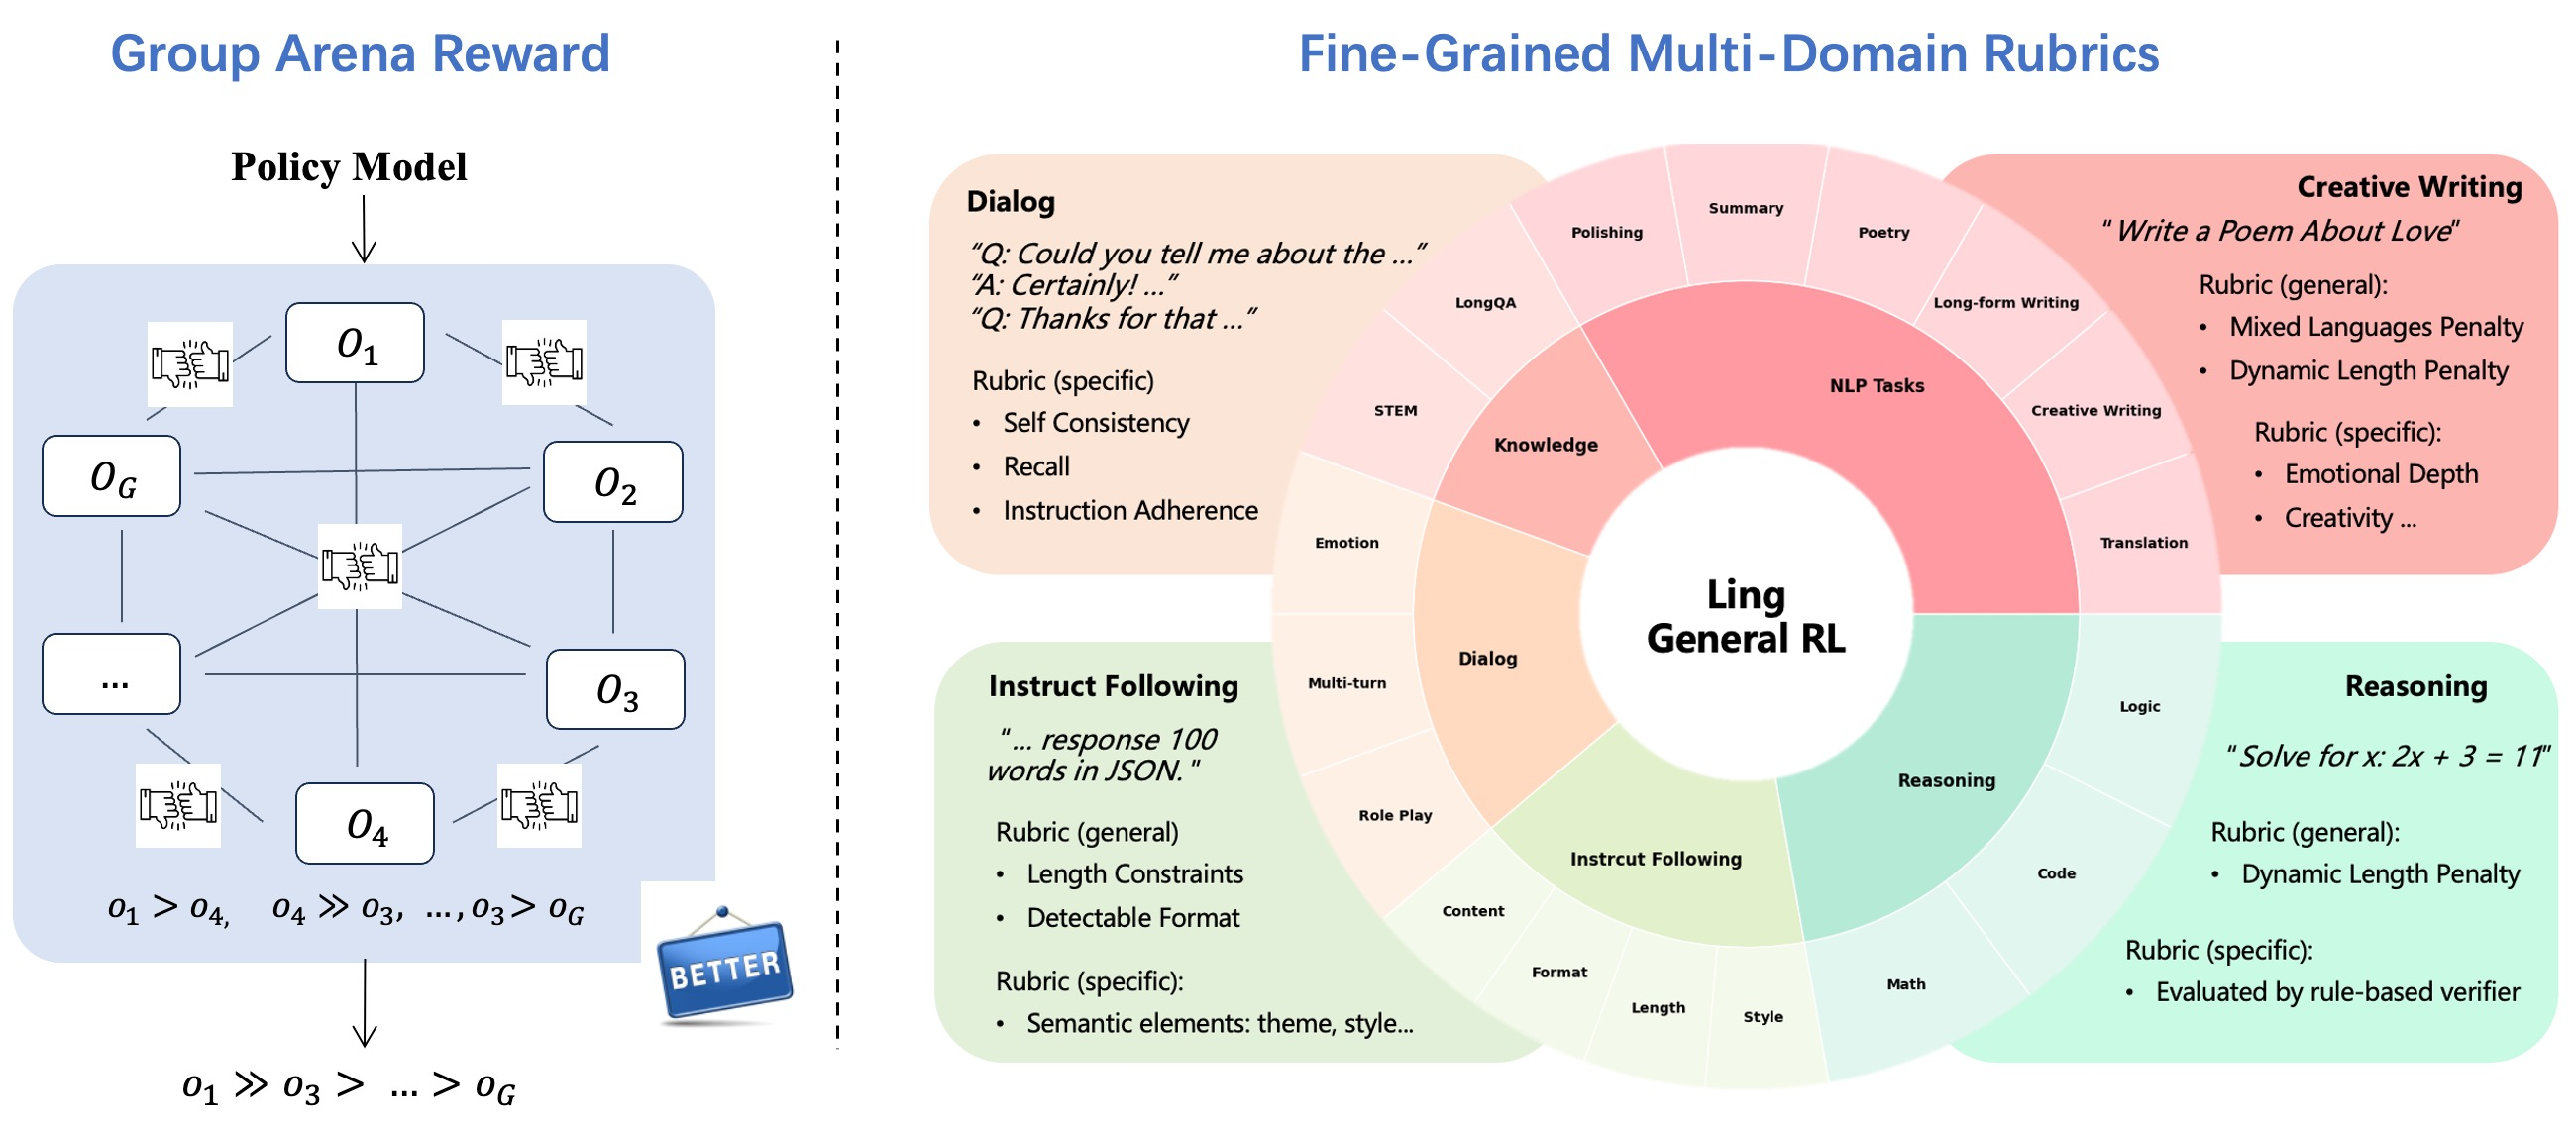
\includegraphics[width=0.95\textwidth]{figs/grl.jpg}
\caption{Illustration of the Group Arena Reward (GAR) mechanism applied to open-ended subjective tasks.}
\label{fig:GAR}
\end{center}
\end{figure}

\subsubsection{Fine-grained Multi-Dimensional RubriX}

To complement GAR with precise preference modeling, we propose \textbf{RubriX}—a domain-extended set of reward evaluation rubrics tailored for subjective general tasks. 
RubriX spans multiple dimensions, including clarity, coherence, creativity, emotional resonance, instruction adherence, and domain-specific accuracy, with instantiations for writing, translation, long-form QA, emotional dialogue, multi-turn conversation, and other instruction-following tasks. 
These structured rubrics guide the reward model to capture subtle aspects of user intent, encouraging responses that are both more natural in flow and more aligned with complex preference criteria.

\subsection{Reward Model System}
To flexibly support reward computation and reward policy orchestration across diverse reasoning tasks within RL training pipelines, we propose a unified scalable reward model system. This system concurrently accommodates rule-based, model-based, and multi-programming-language-based reward verification, scaling to 40K concurrent heterogeneous reward requests with sustained success rates exceeding 99.9\%.

The system architecture comprises three core modules: (1) a highly available sandboxing environment integrating multi-programming-language sandboxes, general reward models inference, visual reward evaluators, and complex environment sandboxes (software engineering, database operations, browser interaction, etc.); (2) a preemptive task scheduling mechanism employing high-performance bounded queues to mitigate timeout-induced failures arising from computational heterogeneity under peak concurrency, achieving a 39\% improvement in system throughput; and (3) an asynchronous reward computation framework that decouples RL training iterations from reward computation latency, yielding empirically measured training time reduction of up to 30\%.








\begin{table}[t]
\centering
    \caption{Comparison between \texttt{Ling-mini-2.0}  and other representative models.}
    \label{tab:results_ling_mini}
    \begin{adjustbox}{width=\linewidth}
    \begin{threeparttable}
    \centering
    \begin{tabular}{lccccc}
    \hline \multirow{2}{*}{\textbf{Benchmark}} & \multirow{2}{*}{\textbf{\splitcell{\texttt{Ling-mini-2.0} }}} & \textbf{\splitcell{Qwen3-4B}} & \textbf{\splitcell{Qwen3-8B}} & \textbf{\splitcell{Ernie-4.5-21B}} & \textbf{\splitcell{gpt-oss-20B}} \\
     &  & \textbf{\splitcell{-Instruct 2507}} & \textbf{\splitcell{(Non-thinking)}} & \textbf{\splitcell{-A3B-PT}} & \textbf{\splitcell{(low thinking)}} \\
    \midrule \multicolumn{6}{c}{\textit{Coding}} \\
    \midrule MBPP Sanitized (Pass@1) & 82.99 & \underline{85.54} & 79.45 & 85.36 & \textbf{89.40} \\
     LiveCodeBench (Pass@1) & \underline{41.69} & 34.03 & 26.10 & 26.10 & \textbf{46.64} \\
     CodeForces (Rating) & \underline{1410} & 1224 & 624 & 480 & \textbf{1481} \\
     BIRD-SQL (Acc.) & \underline{39.60} & \textbf{45.40} & 36.80 & 29.86 & 36.15 \\
     ArtifactsBench & 29.94 & \underline{36.61} & 31.00 & 31.44 & \textbf{45.90} \\
     MultiPL-E (Pass@1) & 70.82 & \textbf{72.03} & 67.37 & \underline{71.92} & 61.10 \\
     FullStack Bench (Pass@1) & \underline{43.45} & 40.37 & 39.24 & 43.02 & \textbf{49.91} \\
    \midrule \multicolumn{6}{c}{\textit{Math}} \\
    \midrule CNMO 2024 (Pass@1) & \textbf{72.66} & \underline{68.49} & 34.38 & 42.71 & 45.31 \\
     AIME24 (Pass@1) & \textbf{65.62} & \underline{64.53} & 27.97 & 24.43 & 45.68 \\
     AIME25 (Pass@1) & \underline{46.72} & \textbf{47.81} & 24.01 & 15.68 & 38.59 \\
     UGMathBench (Acc.) & \underline{66.83} & \textbf{67.14} & 59.62 & 56.31 & 61.57 \\
     Omni-MATH (Acc.) & \textbf{60.30} & \underline{60.25} & 41.71 & 38.71 & 50.70 \\
     HMMT25 (Pass@1) & \textbf{35.83} & \underline{29.79} & 11.46 & 6.88 & 20.05 \\
     FinanceReasoning (Acc.) & 69.64 & \underline{74.17} & 69.52 & 70.55 & \textbf{77.31} \\
     OptMATH (Pass@1) & \textbf{12.20} & \underline{10.39} & \underline{10.39} & 1.51 & 2.71 \\
     Optibench (Pass@1) & \textbf{61.16} & 28.26 & \underline{41.65} & 31.90 & 37.52 \\
     \midrule \multicolumn{6}{c}{\textit{Reasoning}} \\
    \midrule KOR-Bench (Acc.) & 62.00 & \underline{65.12} & 54.40 & 48.48 & \textbf{66.00} \\
     ARC-AGI-1 (Pass@1) & \underline{10.25} & \textbf{15.38} & 4.06 & 0.75 & 3.56 \\
     HLE (Pass@1) & \textbf{6.01} & 4.55 & 4.00 & \underline{5.11} & 4.69 \\
     ZebraLogic (Pass@1) & \textbf{80.20} & \underline{79.50} & 36.05 & 46.98 & 44.10 \\
    \midrule \multicolumn{6}{c}{\textit{Knowledge}} \\
    \midrule GPQA-Diamond (Pass@1) & \underline{58.74} & 44.82 & 48.64 & \textbf{77.27} & 55.71 \\
     C-Eval (Acc.) & \underline{83.31} & 81.71 & 80.06 & \textbf{85.38} & 64.41 \\
     MMLU-Redux (Acc.) & 81.55 & \textbf{84.24} & 80.83 & 82.59 & \underline{83.50} \\
     MMLU-Pro (Acc.) & 65.11 & 62.38 & 52.54 & \underline{65.46} & \textbf{65.59} \\
     MMLU-Pro-Stem (Acc.) & 72.14 & 69.90 & 57.62 & \textbf{72.98} & \underline{72.63} \\
     OlympiadBench-Stem (Acc.) & \underline{70.43} & \textbf{77.53} & 59.37 & 62.17 & 63.02 \\
    \midrule \multicolumn{6}{c}{\textit{Agent}} \\
    \midrule BFCL-V3 (Function Call)\tnote{1} & 53.71 & \textbf{61.16} & \underline{59.50} & -- & 36.22 \\
    \midrule \multicolumn{6}{c}{\textit{Instruction Following}} \\
    \midrule IFEval (Prompt Strict) & 77.74 & \textbf{84.47} & \underline{83.92} & 75.05 & 72.50 \\
    \hline
    \end{tabular}
    \begin{tablenotes}
        \footnotesize
        \item[1] The Ernie-4.5-21B-A3B-PT model lacks function call capability, so BFCL-V3 (Function Call) score is not available for this model.
    \end{tablenotes}
    \end{threeparttable}
    \end{adjustbox}
\end{table}

\begin{table}[t]
\centering
    \caption{Comparison between \texttt{Ling-flash-2.0}  and other representative models.}
    \label{tab:results_ling_flash}
\resizebox{\linewidth}{!}{%
    \centering
\begin{tabular}{lcccccc}
\hline \multirow{2}{*}{\textbf{Benchmark}} & \multirow{2}{*}{\textbf{\splitcell{\texttt{Ling-flash-2.0} }}} & \textbf{\splitcell{Qwen3-32B}} & \textbf{\splitcell{Hunyuan-A13B}} & \textbf{\splitcell{Seed-OSS-36B}} & \textbf{\splitcell{GPT-OSS-120B}} & \multirow{2}{*}{\textbf{\splitcell{GPT-4.1 mini}}} \\
&&\textbf{\splitcell{(Non-thinking)}} & \textbf{\splitcell{-Instruct}} & \textbf{\splitcell{-Instruct}} & \textbf{\splitcell{(low think)}} &  \\
\midrule \multicolumn{7}{c}{\textit{Coding}} \\
\midrule MBPP Sanitized (Pass@1) & \underline{94.17} & 84.78 & 82.82 & 85.42 & \textbf{94.58} & 91.01 \\
 LiveCodeBench (Pass@1) & \textbf{51.38} & 31.50 & 25.77 & 30.73 & 42.68 & \underline{45.54} \\
 CodeForces (Rating) & \textbf{1600} & 696 & 569 & 679 & \underline{1519} & 1309 \\
 BIRD-SQL (Acc.) & \textbf{47.65} & 37.65 & 30.05 & 39.47 & 38.49 & \underline{39.77} \\
 MultiPL-E (Pass@1) & \textbf{75.82} & 70.79 & 68.68 & 69.00 & 33.25 & \underline{73.79} \\
 FullStack Bench (Pass@1) & 47.01 & 48.19 & \underline{50.21} & 45.82 & 46.83 & \textbf{56.31} \\
 Aider-Edit (Acc.) & 71.24 & \textbf{77.82} & 43.80 & 68.05 & 69.17 & \underline{74.44} \\
\midrule \multicolumn{7}{c}{\textit{Math}} \\
\midrule CNMO 2024 (Pass@1) & \textbf{74.48} & 37.41 & 43.84 & 39.58 & \underline{63.72} & 56.68 \\
 AIME24 (Pass@1) & \textbf{69.95} & 29.90 & 32.66 & 23.18 & \underline{57.55} & 51.82 \\
 AIME25 (Pass@1) & \textbf{55.83} & 22.5 & 21.46 & 14.9 & \underline{50.83} & 49.64 \\
 UGMathBench (Acc.) & \textbf{71.90} & 64.10 & 52.10 & 61.87 & \underline{67.58} & 65.65 \\
 Omni-MATH (Acc.) & \textbf{66.64} & 43.81 & 50.11 & 37.35 & \underline{60.39} & 57.32 \\
 HMMT25 (Pass@1) & \textbf{39.58} & 10.42 & 8.54 & 8.33 & \underline{33.54} & 27.86 \\
 FinanceReasoning (Acc.) & 81.59 & 78.51 & 64.27 & 78.14 & \underline{83.84} & \textbf{84.45} \\
 OptMATH (Pass@1) & \textbf{39.76} & 15.51 & 2.86 & 14.61 & 26.96 & \underline{34.49} \\
 Optibench (Pass@1) & \textbf{68.93} & 54.38 & 29.75 & 55.37 & \underline{59.01} & 40.17 \\
\midrule \multicolumn{7}{c}{\textit{Reasoning}} \\
\midrule KOR-Bench (Acc.) & 68.80 & 56.96 & 47.60 & 44.24 & \textbf{73.12} & \underline{70.40} \\
 ARC-AGI-1 (Pass@1) & \textbf{24.56} & 3.31 & 0.06 & 4.38 & \underline{10.69} & 7.62 \\
 HLE (Pass@1) & 5.05 & 4.47 & \textbf{5.68} & 5.15 & \underline{5.33} & 5.10 \\
 ZebraLogic (Pass@1) & \textbf{86.80} & 33.80 & 33.20 & 46.40 & \underline{68.40} & 46.50 \\
\midrule \multicolumn{7}{c}{\textit{Knowledge}} \\
\midrule GPQA-Diamond (Pass@1) & \textbf{68.12} & 56.16 & 52.15 & 51.96 & 63.42 & \underline{66.67} \\
 C-Eval (Acc.) & \underline{87.89} & 87.69 & 76.11 & \textbf{90.00} & 70.94 & 76.90 \\
 MMLU-Redux (Acc.) & \underline{89.34} & 86.88 & 76.50 & 86.56 & 88.50 & \textbf{89.80} \\
 MMLU-Pro (Acc.) & \underline{77.07} & 69.24 & 65.00 & 73.16 & 74.14 & \textbf{77.74} \\
 MMLU-Pro-Stem (Acc.) & \textbf{84.64} & 73.19 & 71.82 & 77.44 & 80.74 & \underline{82.98} \\
 OlympiadBench-Stem (Acc.) & \textbf{87.83} & 72.17 & 63.48 & \underline{76.52} & 73.04 & 72.17 \\
\midrule \multicolumn{7}{c}{\textit{Agent}} \\
\midrule BFCL-V3 (Function Call) & \underline{59.14} & \textbf{63.79} & 54.86 & 39.17 & 58.34 & 56.94 \\
\midrule \multicolumn{7}{c}{\textit{Instruction Following}} \\
\midrule IFEval (Prompt Strict) & 81.52 & \underline{83.73} & 79.11 & 81.52 & 73.2 & \textbf{87.21} \\
\midrule \multicolumn{7}{c}{\textit{Aligment}} \\
\midrule Arena Hard v2.0 (Style-Control) & \underline{49.12} & 28.44 & 7.21 & 33.58 & \textbf{57.34} & 49.10 \\
 Arena Hard v2.0 (Win-Rate) & \underline{61.33} & 34.44 & 8.56 & 37.07 & \textbf{81.19} & 42.77 \\
 Creative Writing v3 & \textbf{85.17} & 77.57 & 59.69 & \underline{82.17} & 79.09 & 74.35 \\
 Writing Bench & \textbf{87.22} & 74.97 & 65.10 & 81.64 & \underline{85.50} & 72.17 \\
Multi-Challenge & \textbf{42.12} & 30.62 & 17.66 & 28.64 & \underline{37.00} & 35.90 \\
\hline
\end{tabular}
}
\end{table}


\begin{table}[t]
\centering
\caption{Comparison between \texttt{Ling-1T}  and other representative models.}
\label{tab:results_ling_max}
\begin{adjustbox}{width=\linewidth}
\begin{threeparttable}
    \centering
\begin{tabular}{lccccc}
\hline \multirow{2}{*}{\textbf{Benchmark}} & \multirow{2}{*}{\textbf{\splitcell{\texttt{Ling-1T} }}} & \textbf{\splitcell{DeepSeek-V3.1-Teminus}} & \textbf{\splitcell{Kimi-K2}} & \multirow{2}{*}{\textbf{\splitcell{GPT-5-main}}} & \textbf{\splitcell{Gemini 2.5 Pro}} \\
 & & \textbf{\splitcell{(Non-thinking)}} & \textbf{\splitcell{-Instruct-0905}} & & \textbf{\splitcell{(lowthink)}} \\
\midrule \multicolumn{6}{c}{\textit{Coding}} \\
\midrule 
 MBPP Sanitized (Pass@1) & \textbf{96.87} & 90.69 & 89.96 & \underline{91.72} & 91.01 \\
 LiveCodeBench (Pass@1) & \textbf{61.68}  & 48.02 & \underline{48.95} & 48.57 & 45.43 \\
 CodeForces (Rating)\tnote{1} & \textbf{1901} & 1582 & 1574 & 1120 & \underline{1675} \\
 BIRD-SQL (Acc.) & \underline{52.38} & 44.88 & 46.45 & 43.97 & \textbf{54.76} \\
 MultiPL-E (Pass@1)\tnote{2} & \textbf{77.91} & \underline{77.68} & 73.54 & 76.66 & 71.48 \\
 ArtifactsBench & \underline{59.31}  & 43.29 & 44.87 & 41.04 & \textbf{60.28} \\
 FullStack Bench (Pass@1) & \textbf{56.55} & \underline{55.48} & 54.00 & 50.92 & 48.19 \\
 Aider-Edit (Acc.) & 83.65 & \underline{88.16} & 85.34 & 84.40 & \textbf{89.85} \\
\midrule \multicolumn{6}{c}{\textit{Math}} \\
\midrule CNMO 2024 (Pass@1) & \textbf{79.25} & 73.78 & 68.92 & 63.11 & \underline{74.65} \\
 AIME24 (Pass@1) & \textbf{80.21} & 71.67 & 67.24 & 67.60 & \underline{77.50} \\
 AIME25 (Pass@1) & \textbf{70.42} & 55.21 & 50.16 & 59.43 & \underline{70.10} \\
 UGMathBench (Acc.) & \textbf{74.95} & \underline{72.70} & 69.97 & 67.27 & 70.10 \\
 Omni-MATH (Acc.) & \textbf{74.46} & 64.77 & 62.42 & 61.09 & \underline{72.02} \\
 HMMT25 (Pass@1) & \underline{47.08} & 41.25 & 38.80 & 36.98 & \textbf{60.73} \\
 FinanceReasoning (Acc.) & \textbf{87.45} & 86.44 & 84.83 & 86.28 & \underline{86.65} \\
 Optibench (Pass@1) & \textbf{74.71} & 64.30 & 60.83 & 40.66 & \underline{68.76} \\
 OptMATH (Pass@1) & \textbf{57.68} & 35.99 & 35.84 & 39.16 & \underline{42.77} \\
\midrule \multicolumn{6}{c}{\textit{Reasoning}} \\
\midrule BBEH (Acc.) & \textbf{47.34} & \underline{42.86} & 34.83 & 39.75 & 29.08 \\
 KOR-Bench (Acc.) & \textbf{76.00} & \underline{73.76} & 73.20 & 70.56 & 59.68 \\
 ARC-AGI-1 (Pass@1) & \textbf{43.81} & 14.69 & \underline{22.19} & 14.06 & 18.94 \\
 ZebraLogic (Pass@1) & \textbf{90.80} & 81.60 & \underline{85.50} & 57.30 & 70.20 \\
 HLE (Pass@1) & 7.60 & \underline{10.38} & 7.29 & 7.33 & \textbf{12.07} \\
\midrule \multicolumn{6}{c}{\textit{Knowlwdge}} \\
\midrule 
 GPQA-Diamond (Pass@1) & 72.98  & \textbf{76.23} & \underline{73.93} & 71.31 & 71.81 \\
C-Eval (Acc.) & \textbf{92.19} & \underline{91.76} & 91.12 & 83.59 & 88.77 \\
 MMLU-Redux (Acc.) & 92.25 & 92.37 & 91.58 & \underline{92.75} & \textbf{94.67} \\
 MMLU-Pro (Acc.) & 82.04 & \textbf{83.25} & 81.03 & 81.94 & \underline{82.13} \\
 MMLU-Pro-Stem (Acc.) & \underline{88.50} & 87.91 & 85.30 & 73.45 & \textbf{88.60} \\
 OlympiadBench-Stem (Acc.) & \textbf{91.30} & 87.83 & 79.13 & 78.26 & \underline{89.57} \\
MedXpertQA (Acc.) & 22.33 & \underline{31.14} & 20.61 & 17.59 & \textbf{44.82} \\	
\midrule \multicolumn{6}{c}{\textit{Agent}} \\
\midrule BFCL-V3 (Function Call) & \underline{69.64} & 52.67 & \textbf{71.05} & 50.27 & 63.31 \\
\midrule \multicolumn{6}{c}{\textit{Instruction Following}} \\
\midrule IFEval (Prompt Strict) & 86.11 & 86.32 & \textbf{90.99} & 85.11 & \underline{87.08} \\
\midrule \multicolumn{6}{c}{\textit{Alignment}} \\
\midrule Arena Hard v2.0 (Style-Control)\tnote{3} & \underline{76.26} & 54.09 & \textbf{76.95} & 68.37 & 65.37 \\
 Arena Hard v2.0 (Win-Rate) & \textbf{75.83}  & 63.24 & 69.88 & 65.06 & \underline{74.46} \\
 Writing Bench & \textbf{89.40}  & 80.95 & \underline{87.59} & 77.07 & 80.53 \\
 Creative Writing v3 & \textbf{89.24} & 85.18 & \underline{87.01} & 80.93 & 84.99 \\
Multi-Challenge & \textbf{58.24} & 42.49 & 48.72 & 48.72 & \underline{51.28} \\
\hline
\end{tabular}
\begin{tablenotes}
        \footnotesize
        \item[1] CodeForces is composed of problems from 14 Div.2 contests along with expert-crafted test cases, while $2209$ representing the highest rating attainable on it.
        \item[2] In MultiPL-E, we choose six programming languages: Python, C++, Java, JavaScript, TypeScript, and PHP.
        \item[3] Arena Hard Style-controlled score following LMSYS’s Arena Hard Auto protocol: https://lmsys.org/blog/2024-08-28/style-control/ .
    \end{tablenotes}
\end{threeparttable}
\end{adjustbox}
\end{table}

\subsection{ApexEval: Searching for Checkpoint with Highest Potential}
\label{ApexEval}

In post-training, RL is used to unlock the model’s reasoning potential. To initialize RL effectively, we must identify the SFT checkpoint with the highest potential. However, conventional methods fall short: 1) They rely on greedy or average pass@k scores, which reflect average performance rather than the best potential; 2) Checkpoints lack strong instruction-following ability, leading to misjudgment of correct responses that deviate from fixed formats.

To address the above two issues with conventional evaluation methods, we propose \textbf{ApexEval} to get the best checkpoint initialization for RL training. The method includes:
\begin{itemize}
    \item Instead of greedy or average pass@k, we use the highest score of pass@k to estimate the probability of producing at least one correct response in multiple attempts, effectively capturing the model's potential upper bound.
    \item To reduce the impact of answer formatting, we use LLM-based intelligent judges (e.g., MathVerify, XVerify) for tasks with explicit answers like mathematics, knowledge, and logic. These judges assess answer validity based on model predictions, minimizing misjudgment caused by pattern variability. For coding tasks, we evaluate valid code snippets via test-case execution to fairly assess actual capabilities.
\end{itemize}


\textbf{Find High-potential Checkpoint.} 
ApexEval is designed to assess a model’s true capability and potential for further improvement. This enables the identification of promising checkpoints for subsequent instruction tuning or RL optimization.
During the Ling 2.0 pretraining phase, we introduce a portion of instant-response and in-depth reasoning data. From a post-training perspective, this inclusion raises the reasoning performance ceiling when applying Evolutionary Reasoning Reinforcement Learning (ERL).

As shown in Figure \ref{fig:apexeval}, we compare Decoupled Fine-Tuning (DFT) with and without Chain-of-Thought (CoT) data during pretraining. The performance ceiling is evaluated using both ApexEval and high-value pass@k metrics. In all settings, pretraining with CoT data consistently yields a higher ceiling under the same DFT configuration.We use ApexEval as the criterion for selecting the initial model for Reasoning Reinforcement Learning. The DFT model pretrained with CoT data exhibits stronger AIME performance at ERL step450 compared to the model without CoT data, indicating a faster performance gain trajectory.

\begin{figure}[h]
\begin{center}	
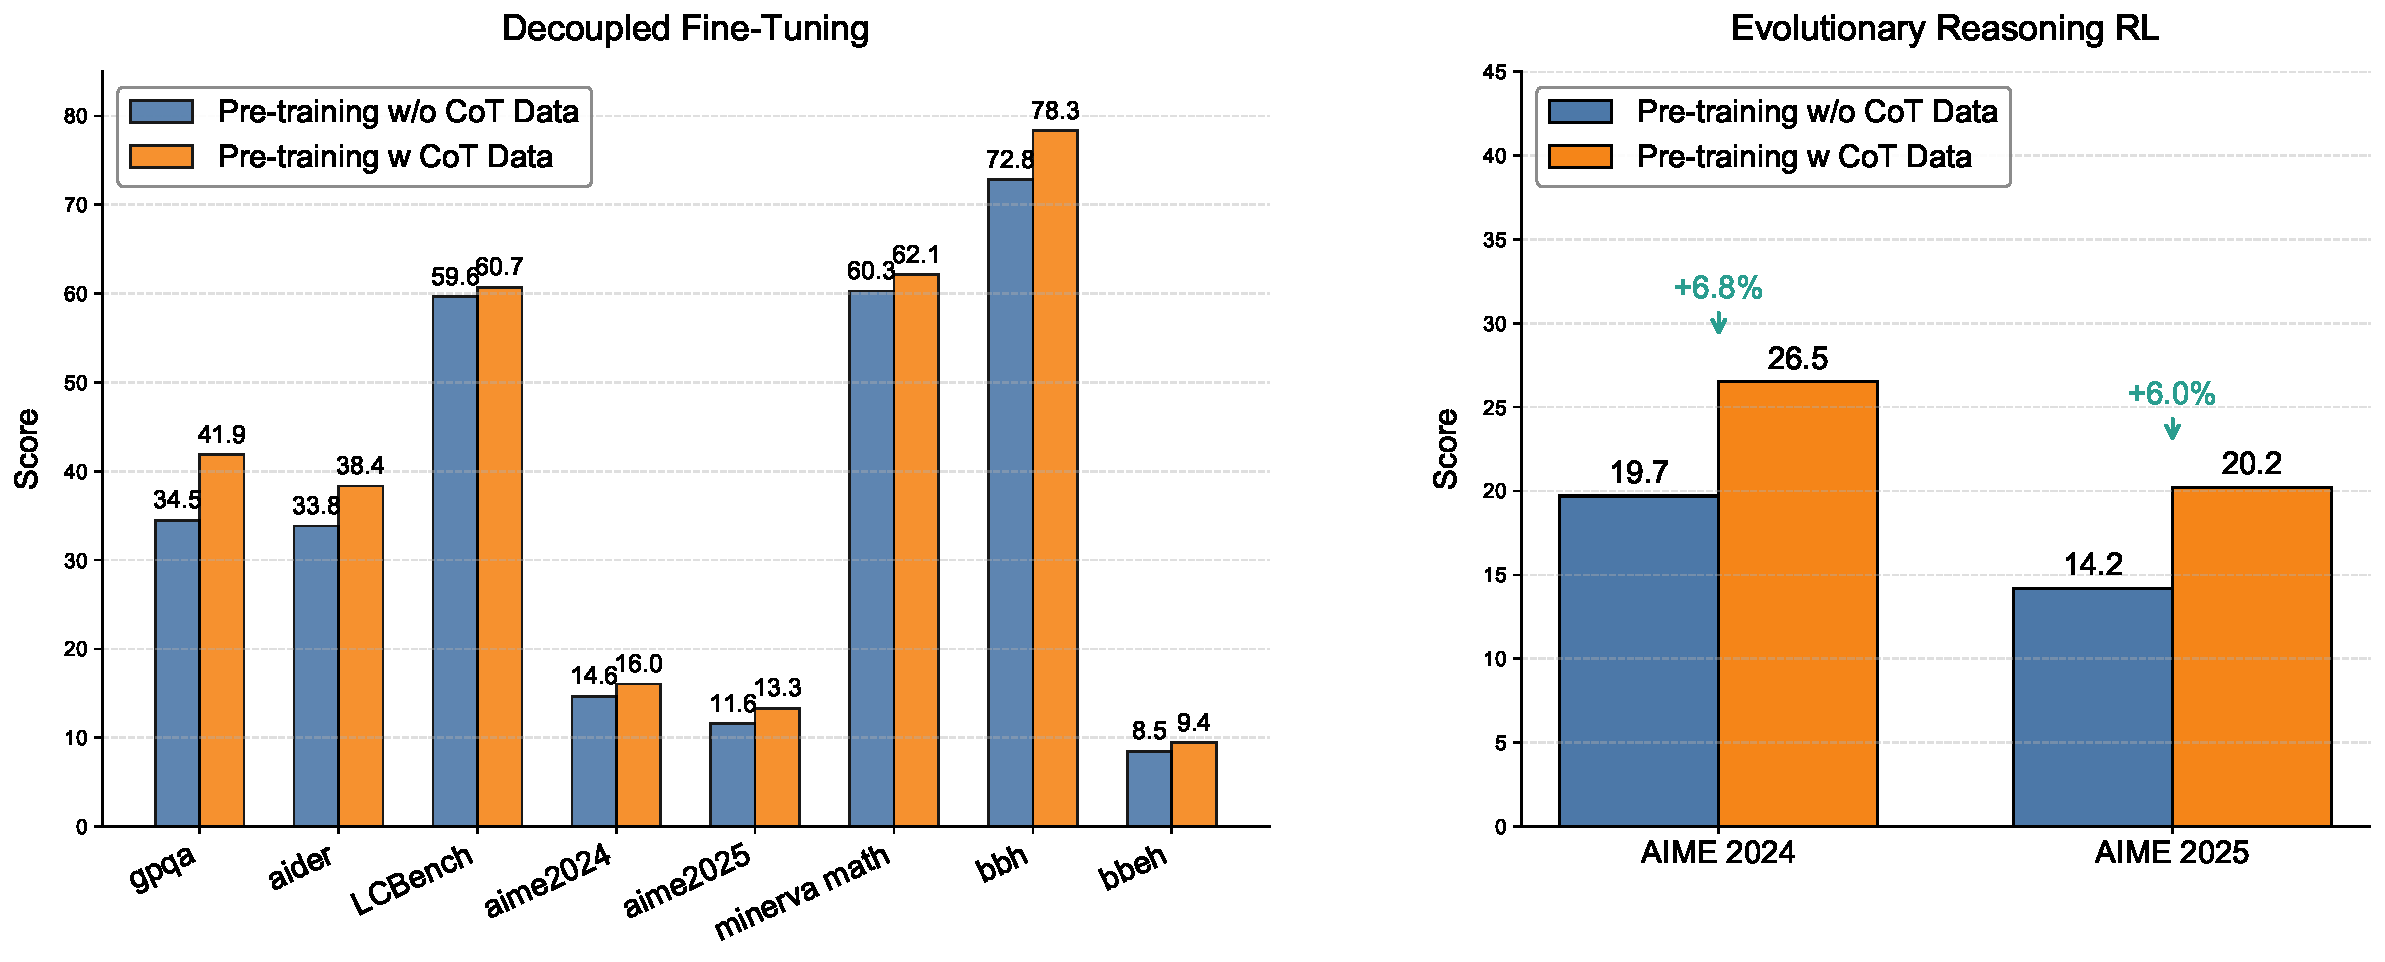
\includegraphics[width=0.8\textwidth]{figs/apexeval_res.pdf}
\caption{ApexEval-based checkpoint selection experiment on the Ling 2.0 mini model. Left: ApexEval results for DFT models pretrained with and without CoT-style data. Right: Performance of the two DFT variants after applying ERL, showing the pretraining-with-CoT model achieves higher AIME scores and faster improvement.}
\label{fig:apexeval}
\end{center}
\end{figure}

\subsection{Evaluation Results}

{\bfseries Benchmarks and Configurations.} 
The suite spans mathematics, coding, reasoning, knowledge, agent, instruction following and alignment ability. Unless noted, we report EM/Acc or Pass@1 with 0-shot prompting and decontamination. For fill-in-the-blank benchmarks, we employ LLM-as-a-Judge to improve the accuracy of the evaluation. The evaluation datasets for post-trained models include 36 benchmarks, which are categorized as follows:
\begin{itemize}
    \item \textbf{Coding Tasks}: MultiPL-E~\citep{cassano2022multipl}, MBPP~\citep{austin2021program}(MBPP Sanitized), LiveCodeBench~\citep{livecodebench}(questions from August 2024 to May 2025), CodeForces~\citep{quan2025codeelo}(ratings from CodeElo), BIRD-SQL~\citep{li2023can}, ArtifactsBench~\citep{artifactsbench}, FullStack Bench~\citep{cheng2024fullstack}, Aider-Edit~\citep{aider}. 
    \item \textbf{Math Tasks}: CNMO 2024~\citep{livemathbench}, AIME24~\citep{aime24}, AIME25~\citep{aime25}, UGMathBench~\citep{xu2025ugmathbench}, Omni-MATH~\citep{omni-math}, HMMT25~\citep{HMMT25}, FinanceReasoning~\citep{FinanceReasoning}, Optibench~\citep{optibench}, OptMATH~\citep{optmath}. For the Omni-MATH benchmark, instead of the original rule-based evaluation method, we rely on LLM to perform the assessment.
    \item \textbf{Reasoning Tasks}: BBEH~\citep{bbeh}, KOR-Bench~\citep{korbench}, ARC-AGI-1~\citep{arc-agi}, ZebraLogic~\citep{zebralogic}, HLE~\citep{hle}. For BBEH, we employ LLM-as-a-Judge for evaluation. For ARC-AGI-1, ZebraLogic and HLE, we repeat each query 4 times and report the Pass@1 score. 
    \item \textbf{Knowledge Tasks}: C-Eval~\citep{ceval},  MMLU-Redux~\citep{mmlu}, MMLU-Pro~\citep{mmlu-pro}, GPQA-Diamond~\citep{gpqa}, MMLU-Pro-Stem~\citep{mmlu-pro}, OlympiadBench-Stem~\citep{he2024olympiadbench}, MedXpertQA~\citep{zuomedxpertqa}. For GPQA-Diamond, we repeat 16 times for each query and report the Pass@1 score. For MMLU-Pro-Stem, we selected a subset of the mmlu-pro evaluation set belonging to the STEM category, consist of math, physics, chemistry, engineering, biology, computer science, and calculated their average score. For the OlympiadBench-Stem evaluation set, we selected the physics subset from OlympiadBench~\citep{he2024olympiadbench} that is suitable for evaluating language models, excluding subsets containing images.
    \item \textbf{Alignment Tasks}: Arena Hard v2.0~\citep{li2024crowdsourced,arenahard2024}, Writing Bench~\citep{wu2025writingbench}, Creative Writing v3~\citep{creative-writing-bench-v3}, Multi-Challenge~\citep{deshpande-etal-2025-multichallenge}.
    \item \textbf{Agent\&Instruction Following Tasks}: BFCL-V3~\citep{berkeley-function-calling-leaderboard}, IFEval(Prompt Strict)~\citep{zhou2023instruction}.
\end{itemize}

Table \ref{tab:results_ling_mini}, Table \ref{tab:results_ling_flash} and Table \ref{tab:results_ling_max} provide comprehensive comparisons of \texttt{Ling-mini-2.0} , \texttt{Ling-flash-2.0} and \texttt{Ling-1T}  against leading models. As shown in Table \ref{tab:results_ling_max}, \texttt{Ling-1T}  demonstrates superiority over leading models across multiple domains, including coding, math, reasoning, alignment and multi-turn dialogues on the majority of benchmarks. Current results of the \texttt{Ling-1T}  align well with the scaling law. Moreover, we have the following findings:

\textbf{Reasoning Capability.} 
Benefits from the In-depth Reasoning during the Decoupled Fine-tuning phase and evolutionary CoT training during RL, the reasoning capability of the model significantly improve.
Respectively,  the in-depth Reasoning in SFT employs prompts in Table.\ref{tab:dft_response_modes} to establish a dedicated deep-reasoning mode, providing a robust foundation for RL, 
while the evolutionary CoT in subsequent RL instill adaptive reasoning in reflex-grade non-thinking models, enabling them to scale their reasoning depth according to problem complexity.
As shown in 
Table \ref{tab:results_ling_mini}, Table \ref{tab:results_ling_flash} and Table \ref{tab:results_ling_max}, the \texttt{Ling-mini-2.0}, \texttt{Ling-flash-2.0} and \texttt{Ling-1T} outperform most of the leading industry models in various benchmarks that require reasoning capability, involving coding tasks e.g. LiveCodeBench, MBPP Sanitized and CodeForces, math tasks e.g. CNMO 2024, Omni-MATH and OptMATH, and reasoning tasks e.g. BBEH, KOR-Bench and ZebraLogic.



\begin{figure}[htp]
    \centering
    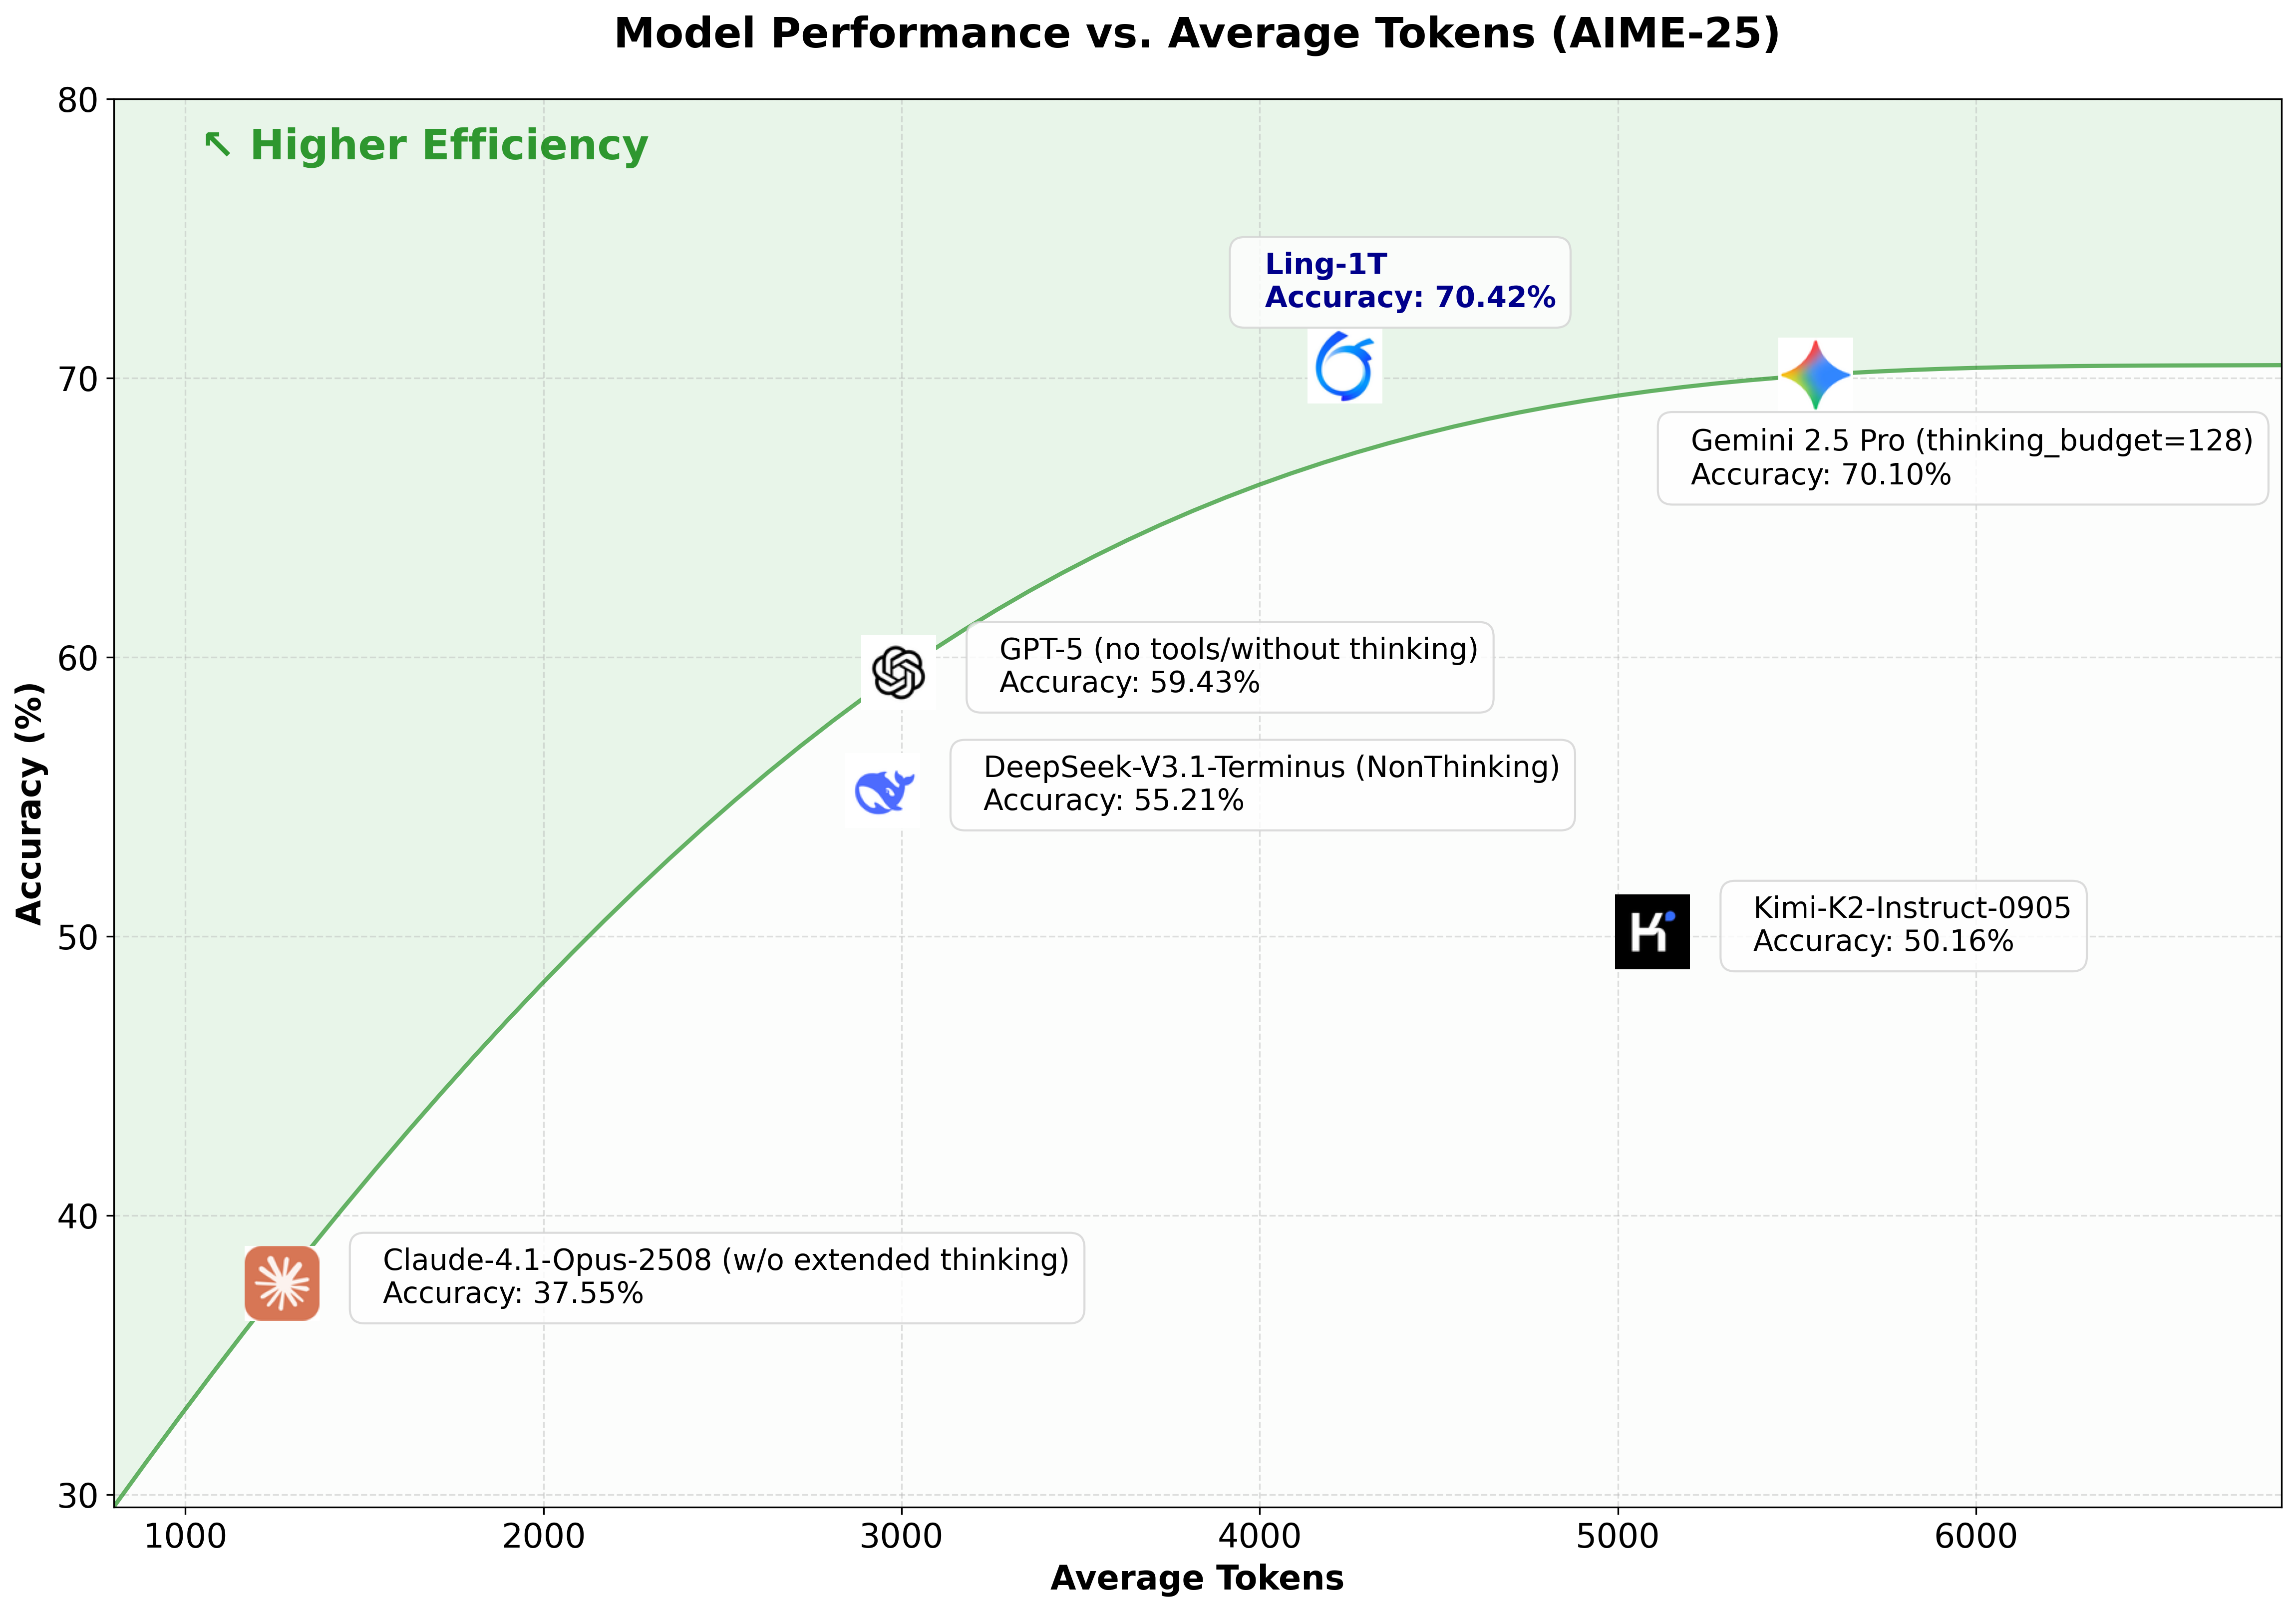
\includegraphics[width=0.8\linewidth]{figs/aime_25_average_tokens.png}
    \caption{Model Performance vs. Average Tokens (AIME-25)}
    \label{fig:aime_25_average_tokens}
\end{figure}

\textbf{Better and Cheaper.}
We analyze the overall performance of \texttt{Ling-1T}  in terms of reasoning accuracy and efficiency. As illustrated in Figure \ref{fig:aime_25_average_tokens}, taking the competition-level mathematics benchmark AIME 25 as an example, \texttt{Ling-1T} showcase its advantage in "efficient thinking and precise reasoning." 
The optimal balance between efficient thinking and precise reasoning benefits from the evolutionary CoT. It progressively activates the model's reasoning ability from shallow to deep, while enabling precise control over reasoning costs. We believe that for reflexive non-thinking models, this approach—gradually activating reasoning capability from pre-training to post-training—can continuously push the Pareto frontier of reasoning accuracy and average reasoning depth.
